\documentclass[a4paper,12pt]{report}
\usepackage[utf8]{inputenc}
\usepackage{times}
\usepackage{graphicx}
\usepackage{url}
\usepackage{amsmath}
\usepackage{array}
\usepackage{mathtools}
\usepackage{ifthen}
\usepackage{mathrsfs}
\usepackage{setspace}

\oddsidemargin 0.1in		% Left margin is 1in + this value
\textwidth 5.75in		% Right margin is not set explicitly
\topmargin 0in			% Top margin is 1in + this value
\textheight 8.5in			% Bottom margin is not set explicitly
%\setlength{\columnsep}{2cm}



\iffalse
These words need to be added to the dictionary:
Ginzburg, soliton, Runge, Kutta, CGLE, Fourier, Landau
discretise nonlinear

I will use nonlinear (not non linear or non-linear)
\fi


\iffalse
\begin{figure}[h]
\centering
\includegraphics[width=4.6in]{correlation}
\caption{A ploperature.}
\label{corr} 
\end{figure}
\fi


\iffalse
Before I submit, make sure I check that the following have updated themselves properly.
Spell Check
Contents Page
Image reference numbers
Table reference numbers
Citation numbers
\fi






\begin{document}
\begin{titlepage}
\centering
{\ \\ }
\vspace{3cm}
{\bf  \fontsize{1.35cm}{2.5cm}\selectfont \vspace{0.5cm} Classifying Solutions\vspace{0.5cm} of \vspace{0.5cm} the Complex Ginzburg \vspace{0.5cm}Landau Equation with Machine Learning\vspace{0.5cm}}\\
%\vspace{2cm} \\
{\Huge By Max Proft}\\
{\Huge u5190335}
\end{titlepage}










\newcommand{\unnum}[2]{
\ifthenelse{\equal{#1}{chapter}}{\chapter*{#2}}{
\ifthenelse{\equal{#1}{section}}{\section*{#2}}{
\ifthenelse{\equal{#1}{subsection}}{\subsection*{#2}}
{\chapter*{ERROR: #2}}}}
\addcontentsline{toc}{#1}{#2} 
}%This is the exception if no case matches!!!
\tableofcontents{}
\iffalse
The order is:
Chapter
Section
Subsection
Subsubsection (not shown in contents)
\fi



\onehalfspacing


\unnum{chapter}{Abstract}
Make this half a page \\\\
Produced a program to generate solitons.
The energy difference, frequency, height difference and width were recorded for a large number of parameters (30,000 different values) and an attempt was made to be able to use machine learning to predict these. The reason we want to do this is because typically classifying regions is done by hand, and so it is difficult to see the boundary of one region of solitons (e.g. exploding) is. This was unsuccessful. 


\unnum{chapter}{Acknowledgements}
Chuck in some very cliché acknowledgements here.
Thanks Nail and Adrian for helping me, etc. 

\unnum{chapter}{List of Figures}

\unnum{chapter}{What to add}
Non uniqueness of solitons - Creeping vs oscillating. I think I have examples of oscillating an non oscillating.
\\\\
Do I want equation numbers?




\chapter{Introduction to the CGLE}
%The purpose of this chapter is to introduce the equation, explain what all the terms represent, and 
The Complex Ginzburg Landau equation (CGLE) is a differential equation that is typically written in the following form, but also it is often written without the quintic terms ($|\psi|^4\psi$): 
$$i\psi_t +\frac{D}{2}\psi_{xx}+|\psi|^2\psi +\nu |\psi|^4\psi = i\delta \psi+i\epsilon|\psi|^2\psi +i\beta\psi_{xx}+i\mu|\psi|^4\psi$$
$\psi$ refers to the normalised field (normalised with respect to what?)\\
$D = \pm 1$. if $D=1$ then normal. This means that as the optical frequency increases, the group velocity decreases. If $D=-1$ then the group velocity dispersion is anomalous, which is the opposite.\\
$\beta>0$ is parabolic gain and $\beta<0$ effectively means that sharp spikes are filtered out. (This doesn't make sense - shouldn't it be the other way around?)
 causes spectral filtering\\
$\delta$ is the linear gain/loss depending on whether it is positive/negative. \\
$\epsilon$ is nonlinear gain which can arise for a variety of reasons, such as saturable absorption (absorption decreases/reflectivity increases as intensity increases.)\\
$\mu$ and $\nu$, when negative, represents the saturation of the NL gain and NL refractive index respectively. 
\\\\
This equation describes the evolution of a number of systems, from quantum systems like fibre optic propegation in mode locked lasers, superconductivity, superfluidity, as well as classical systems like Bernard Reyleigh convection.
It is an amplitude equation, which means that the quantity we are modelling (e.g. temperature) is given by the amplitude of $\psi$, albeit with scaling. 



\section{Applications and pseudo-derivation}
The CGLE describes a wide range of phenomena. Upon setting various components to zero, we get can derive a number of equations in fluid dynamics, such as the diffusion equation, as well as the nonlinear Schr\"odinger equation. 
On top of this, Aranson and Kramer (world of CGLE) give a method to transform a general set of hydrodynamic equations to the CGLE. This hydrodynamic equation is given as:
$$\tau (\partial_{\tilde t}\tilde A-\tilde v_g\cdot \tilde\nabla \tilde A)=\epsilon(1+ia)\tilde A+\xi^2+(1+ib)\tilde\nabla^2 \tilde A-g(1+ic)|\tilde A|^2 \tilde A$$ 
Aranson amd Kramer tell us that we can rescale the axes in order to get the CGLE back. 
$$\tilde A=(\epsilon/g)^{1/2} A \ exp[-i (\epsilon a/\tau)\tilde t], \ \ \tilde t = (\tau/\epsilon)t, \ \ \vec {\tilde x} = (\xi/\epsilon^{1/2})\vec x+\vec v_g \tilde t$$
This substitution yields the cubic CGLE in the following form:
$$\partial_t A=A+(1+ib)\nabla^2A-(1+ic)|A|^2A$$


Rayleigh-Benard convection:
step 1: it obays the swift hohenberg equation. \\
step 2: if the convection cells are symmetric, then it needs to be invariant under $x\rightarrow -x$  and so the simplest nonlinearities we can have are $x^3$ and $x^5$. We can also then assume that the field satisfies $U=F[z] e^{\sigma t+iqx}+cc$, where sigma is the growth rate, q wavenumber, cc is the complex conjugate. 
step 3: subbing this into the swift hohenberg equation, and assuming nonlinearities are small, the growth rate is given by $\sigma = \epsilon -D(q_c^2-q^2)^2$
step 4: make assumptions such as $q\approx q_c$ for small $\epsilon$ and expand and simplify for the amplitude equation which gives the CGLE.
\\\\
If we want a general differental equation of a complex parameter which is invariant under multiplication by a phase shift $e^{i\phi}$, then we have limited choices of parameters.
Any derivative is fine.You can get rid of first order derivatives in x by rescaling the parameter $x$. and if we assume that diffusion is dominant, we can ignore higher order derivatives. 
\\\\
Additional terms could be approximated with elements from $\{A,A^*, A^*A, AA^*A,A^*AA^* ...\}$, and so to be able to satisfy the invariance under phase shift, we would expect terms of the form $|\psi|^{2n}\psi$ for some positive integer n. 
\\\\
superconductivity has energy given by $F=F_n +\alpha |\psi|^2+\frac{\beta}{2}|\psi|^4 +\frac{1}{2m}|(-i\hbar\nabla -2eA)\psi|^2+\frac{|B|^2}{2\mu_0}$, where $B=\nabla \times A$ is the magnetic field and vector potential. This is the energy when near a superconducting transition If there is no magnetic field.
\\\\
We then say that the evolution equation is given by:Lyapunov functional http://pauli.uni-muenster.de/tp/fileadmin/lehre/NumMethoden/SoSe10/Skript/GLE.pdf
$$\partial_t \psi = -\frac{\delta F}{\delta A^*} F $$
Invariance under a phase shift, and invariant under a reflection.
superfluidity,
and Bose-Einstein condensation to liquid crystals
\\\\
THIS IS COPPIED FROM TWOTCGLE, but explains to me why it is so common.
It provides a reduced, universal description of
weakly nonlinear spatio-temporal phenomena in ex-
tended (in x  ) continuous media whose linear dispersion
is of a very general type (see below) and that are invari-
ant under a global change of gauge [multiplication of A
by $exp(i\phi)]$. This symmetry typically arises when A is
the (slowly varying) amplitude of a phenomenon that is
periodic in at least one variable (space and/or time) as a
consequence of translational invariance of the system.
END COPY
\\\\
On the first page of TWOTCGLE, he gives an example hydrodynamic equation. We see the convection-diffusion equation in part of this. Also the navier stokes is hidden in here as well. Double diffusive convection, Rayleigh Benard convection
\\\\
COPIED:
he CGLE may also be viewed as a dissipative exten
sion of the conservative nonlinear Schrodinger equation,
END COPIED
\\\\
Thngs to llok at:
There is an extensive mathematical literature on the
CGLE, which we shall only touch upon; see, for ex-
ample, Doering et al. (1987, 1988); van Harten (1991);
Schneider (1994); Doelman (1995); Mielke and
Schneider (1996); Levermore and Stark (1997); Mel-
bourne (1998); Mielke (1998).
\\\\
Sinks and sources
\\\\
I should also add in something about fibre optic propegation as well, as a lot of the papers i use reference this.
\\\\
I don't think my sequence is right. Instead the taylor series should give the terms $\{A^n {A^*} ^m\}$, but we still get rid of the terms that don't satisfy the desired properties.
\\\\
Put in a picture to explain rayleigh-bernard convection, 


\chapter{Mathematical Theory Behind Solving the CGLE}

\section{A Brief look at Different Methods to solve the CGLE}

A finite difference method was used initially to get it all going. This is bad because you do $\delta \psi / \delta x$, so over a small time period, the $\delta \psi$ term can lose several digits of precision, not good. There are a number of other ways for this to be solved though. 
\\\\ 
For the nonlinear schrodinger equation, (Taha and Ablowitz) compared various methods for solving this. While under certain conditions, some other methods were found to be better than the split step fourier method, overall it was found to be a faster algortihm. Given that the CGLE is an extension of the NLSE, this means that this should also be a reasonably good method to do this part as well. This has previously been done by other authors as well, (Wang, Zhang).

\section{Split Step Fourier and Runge-Kutta Method}
Note that in the following section, we are instead going to treat the CGLE as being the following equation which we break into linear and nonlinear parts:
$$\frac{d\psi}{dt} = A \frac{d^2\psi}{dx^2} + B\psi + C |\psi|^2\psi + D|\psi|^2\psi = \hat L \psi + \hat N \psi$$
where the linear component is:
$$\hat L \psi = A \frac{d^2\psi}{dx^2} + B\psi$$
and the nonlinear component is:
$$\hat N \psi = C |\psi|^2\psi + D|\psi|^2\psi$$

\subsection{Linear evolution (Fourier)}
Here we are solving the equation: 
$$\frac{d\psi}{dt}=A\frac{d^2\psi}{dx^2}+B\psi$$
Defining the fourier transform by: 
$$\hat \psi(f)=\int\limits_{-\infty}^\infty \psi(x)e^{-i2\pi x f} dx$$
By taking the fourier transform of both sides, the equation becomes:\\
$$\frac{d \hat \psi}{dt}= (-2\pi i f)^2 A \ \hat \psi (f)+B\ \hat \psi(f)= (B-A \ 4 \pi^2 f^2) \hat \psi(f)$$
$$\implies \hat \psi_t(f) = e^{(B-A \ 4\pi^2 f^2)t}\hat \psi_0(f)$$
And so upon inverse fourier transforming, we get the solution to this DE, where $\hat \psi_t(f)$ is the fourier transform at time $t$.
The Fourier transform can be done numerically with a discrete fourier transform, as described in a later subsection.

\subsection{Nonlinear evolution (Runge-Kutta)}
Here we are solving the equation:
$$\frac{d\psi}{dt}=C|\psi|^2\psi + D|\psi|^4\psi$$
The runga kutta method allows you to numerically solve a 1st order differential equation. which are of the form $\frac{dy}{dt}=f(t,y)$. Similar to Euler's method (which is basically just doing a derivative from first principles), except that the runge kutta method has better convergence than this. (it goes as $h^5$ as opposed to Euler's Method which is $h^2$, the backward euler formula, $h^2$, or improved euler formula which goes as $h^3$. Here $h$ is the step size. 
\\\\
The steps for doing this are as follows:
Step 1: define $f(t,y)=f(y)=C|y|^2 y  +D|y|^4 y$
Step 2: Have an initial value for $t$ and $y$, and step size and number of steps
Step 3: define the following:
$$K_1 =f(t,y)=f(y)$$
$$K_2 =f(t+0.5h,y+0.5*h*K_1)=f(y+h*K_1/2)$$
$$K_3 =f(t+0.5h,y+0.5*h*K_2)=f(y+h*K_2/2)$$
$$K_4 =f(t+h,y+h*K_3)=f(y+h*K_3)$$
Step 4: we then progress forwards $t$ and $y$ in the following way:
$$t\rightarrow t+h$$
$$y\rightarrow y+(K_1+2K_2+2K_3+K_4)*h/6$$






\iffalse
\subsection{The relationship between a Fourier Transform and a Discrete Fourier Transform}
I am pretty sure this entire section needs to be rewritten.\\
We can approximate any function with a Fourier series. (by applying periodic boundary conditions)\\
$$f(t)=\sum\limits_{-\infty}^{\infty} c_n e^{i n t}$$
Multiplying both sides by $e^{-i m t}$ and integrating from 0 to $2\pi$, and dividing by $2\pi$:
$$\frac{1}{2\pi} \int\limits_{0}^{2\pi} f(t)e^{-i m t}dt = \frac{1}{2\pi} \sum \limits_{n=-\infty}^{\infty} c_n \int\limits_{0}^{2\pi} d^{i (n-m) t} dt= c_m$$
$$\frac{1}{2\pi} \int\limits_{0}^{2\pi} f(t)e^{-i m t}dt =c_m$$
We use the substitution:
$$t = \frac{2\pi}{L}  x \implies x = \frac{L}{2\pi} t$$
$$dt = \frac{2\pi}{L}  dx$$
And then this becomes:
$$c_m = \frac{1}{L} \int\limits_{0}^{L} f(x) e^{-i m 2\pi x/L} dx $$

For a fourier series $\{c_n\}$, the fourier transform is given given by:

$$\hat f (freq) = \sum\limits_{-\infty}^{\infty} c_n \mathscr{\hat F}(e^{i n 2 \pi x/L})(freq)$$ 

But we have $$\mathscr{\hat F}(e^{i n 2 \pi x/L}) = \int\limits_{-\infty}^\infty e^{i n 2 \pi x/L}e^{-i 2\pi freq x} dx $$
$$= \int\limits_{-\infty}^\infty e^{i x (n 2 \pi /L - 2\pi freq )}dx = 2\pi \delta (n 2\pi/L -2\pi freq)= \delta (n /L - freq)$$

And so we get:
$$\hat f (freq) = \sum\limits_{-\infty}^{\infty} c_n \delta(freq.- n/L)$$
$$= \sum\limits_{-\infty}^{\infty} c_n /L \delta(freq. L- n)$$

If we inverse fourier transform we get the following.
We can also use $x/L=n/N$
$$Data = spacial,  Fata=frequency$$


I don’t think the following is useful:
$$f(x)= \sum\limits_{n=-\infty}^\infty f_n e^{2\pi i n x/L} $$
If we multiply both sides by $e^{-2\pi i m x/L}$ and integrate we get:
$$\int \limits_{-\infty}^\infty f(x)e^{2\pi i n x/L} dx = \sum\limits_{n=-\infty}^\infty  f_n  \int \limits_{-\infty}^\infty  e^{i 2 \pi x/L (n-m)} dx  =  \sum\limits_{n=-\infty}^\infty  f_n  \int \limits_{-\infty}^\infty  e^{i 2 \pi x (n-m)/L} dx  $$
$$=  \sum\limits_{n=-\infty}^\infty  f_n \delta((n-m)/L) = f_n \delta((n-m)/L)$$
\fi




\subsection{The relationship between a Fourier Transform and a Discrete Fourier Transform:}
Below works for periodic boundary conditions, or if you assume that the function goes to zero at the boundary. For ease of proving the relationship, we assume the latter. 
\\\\
Defining the Fourier transform as:
$$\tilde \psi(f) = \int_{-\infty}^\infty \psi(x) e^{-i2\pi xf} dx \approx \int_0^L\psi(x)e^{-i2\pi x f}dx$$
Let $\Delta x=L/N$ for some integer $N$.
$$\approx \sum\limits_{n=0}^{N-1}\psi(n \Delta x) e^{-i 2\pi n \Delta x f}\Delta x$$
With the same arguments, we get the inverse Fourier transform to be:\\ 
($\Delta f = (f_1-f_0)/N$, for some values of $f_1$ and $f_2$)
$$\psi(x) = \int_{-\infty}^\infty \tilde\psi(f)e^{i 2\pi x f} df \approx \int_{f_0}^{f_1}\tilde\psi(f)e^{i 2\pi x f}df \approx \sum\limits_{m=0}^{N-1}\tilde\psi(f_0+m\Delta f)e^{i 2\pi n\Delta x f_0} e^{i 2\pi x m\Delta f}\Delta f$$
Let $\psi(n\Delta x) = \psi_n$ and $\tilde\psi(f_0+m\Delta f) = \tilde \psi_m$ and let $f_0=-\pi/\Delta x$ 
$$\tilde \psi_m\approx \Delta x \sum\limits_{n=0}^{N-1}\psi_n e^{-i 2\pi n \Delta x f_0}e^{-i 2\pi n m \Delta x \Delta f}$$
$$\psi_n  \approx \Delta f e^{i 2\pi n\Delta x f_0}\sum\limits_{m=0}^{N-1}\tilde\psi_m e^{i 2\pi n m \Delta x \Delta f}$$
Since the definition of the discrete Fourier transform is
$$\tilde A_m =  \sum\limits_{n=0}^{N-1} A_n e^{-i 2\pi n m/N}$$
$$A_n  = \frac{1}{N}\sum\limits_{m=0}^{N-1}\tilde A_m e^{i 2\pi n m/N}$$
We now have a way to compute (inverse) Fourier transforms given a set of data that is a sufficiently good approximation of the initial function.
\\\\
We want $f_1-f_0=1/\Delta x$ so that the frequency difference corresponds to the difference between adjacent elements. This means we get $\Delta f = 1/(N\Delta x)$. We then choose to take $f_0=\frac{-1}{2\Delta x}$ is chosen so it satisfies the Nyquist limit.
$$\tilde \psi_m\approx \Delta x \sum\limits_{n=0}^{N-1}\psi_n e^{i \pi n }e^{-i 2\pi n m/N}=\Delta x \sum\limits_{n=0}^{N-1}\psi_n (-1)^n e^{-i 2\pi n m/N}$$
$$\psi_n  \approx \frac{e^{-i \pi n}}{N\Delta x}\sum\limits_{m=0}^{N-1}\tilde\psi_m e^{i 2\pi n m/N}=\frac{(-1)^n }{N\Delta x}\sum\limits_{m=0}^{N-1}\tilde\psi_m e^{i 2\pi n m/N}$$


\subsection{Combining these operations}
With the split step fourier method, we assume that the linear and nonlinear terms do not affect each other over short timescales. This means that we can propegate forwards according to the linear evolution equation, and then propegate forwards according to the nonlinear evolution equation, and we should get a good approximation for the solution to the original differential equation. This can be represented as the following, where $\hat N$ refers to the nonlinear evolution operator, and $\hat L$ refers to the linear evolution operator.
$$\psi(t)=e^{\hat N(t)}e^{\hat L(t)}\psi(0)$$ 
It turns out, however, that a more stable way of doing this evolution is with the following (notice that the two outside terms are both evolution operators for half of the time period):
$$\psi(t)=e^{\hat N(t/2)}e^{\hat L(t)}e^{\hat N(t/2)}\psi(0)$$ 


Baker Campbell Hausdoff
Lie Product Formula
Trotter Product Formula



\section{Testing the Code}
I compared with mathematica and got the same answer with initial conditions ------ and step size ------ for both the linear and NL parts.\\
Also I subbed in exact solns to the NLSE and it matched.\\
Upon decreasing the step size, if the solution doesn't change significantly, we expect a very similar answer. \\
\\
Additionally, as previously done, there are a number of papers which give interesting solutions to the CGLE, and we can reproduce these solitons.









\chapter{Types of solitons}
You need to wait for the transient response to go away, and keep the rest (only interested in the long term behaviour)
\\\\
There are many types of solitons, however an explicit expression for the function usually cannot be found. 

While many explicit solutions for the schrodinger equation have been found, with additional nonlinearity means that finding explicit solutions to the CGLE is often not possible.
\\\\
(Jia-Min Zhu and Zheng-Yi Ma (2007),Pierre Hillion (2012), Mihalache and Panoiu (1992), Yan-Ze Peng and Krishnan (2007) =  Schrodinger equation)
\\\\
We can classify solitons depending on their behaviour.
Stationary solitons maintain a constant amplitude.
Pulsating solitons are another type, and can be categorised into subsets such as "plain pulsating",  "exploding" and creeping. \\\\
Plain pulsating solitons are periodic and don't exhibit any significant features, as given in figure \ref{plain}.
\begin{figure}[h]
\centering
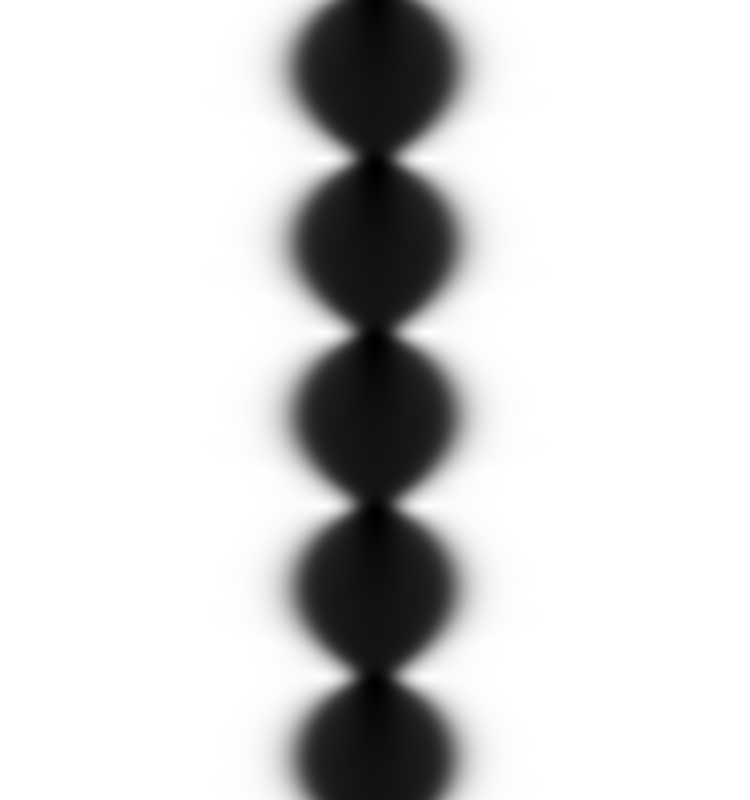
\includegraphics[width=2.6in]{plain}
\caption{The 2D plot of a plain pulsating soliton with parameters ..........}
\label{plain} 
\end{figure}
Exploding solitons are characterised by a sharp jumps in their energy profile, as given in figure \ref{expl_profile}, with the 2D intensity given in figure \ref{expl}. Other solitons will, instead of exploding outwards, give a high intensity spike, as in figure \ref{highamp} whose energy increases by >10 times because of the spike
\begin{figure}[h]
\centering
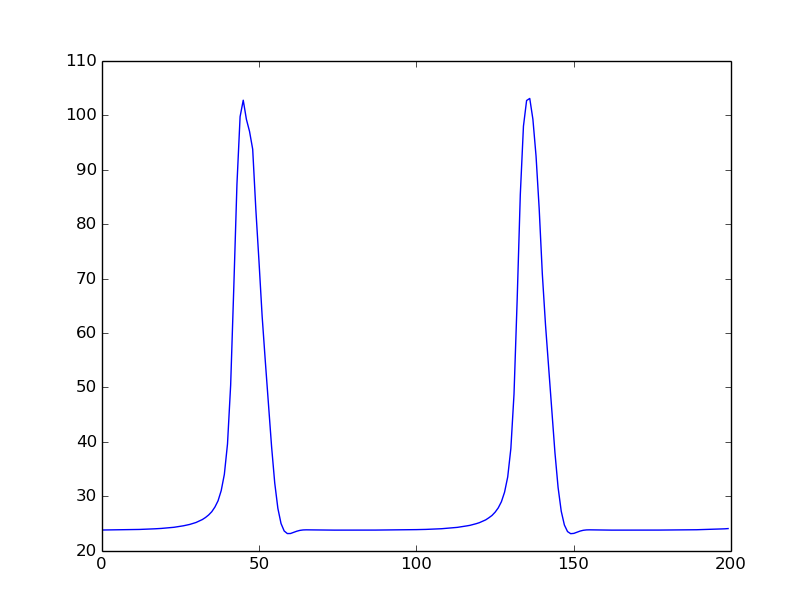
\includegraphics[width=2.6in]{expl_profile}
\caption{The profile of an exploding soliton with parameters ..........}
\label{expl_profile} 
\end{figure}
\begin{figure}[h]
\centering
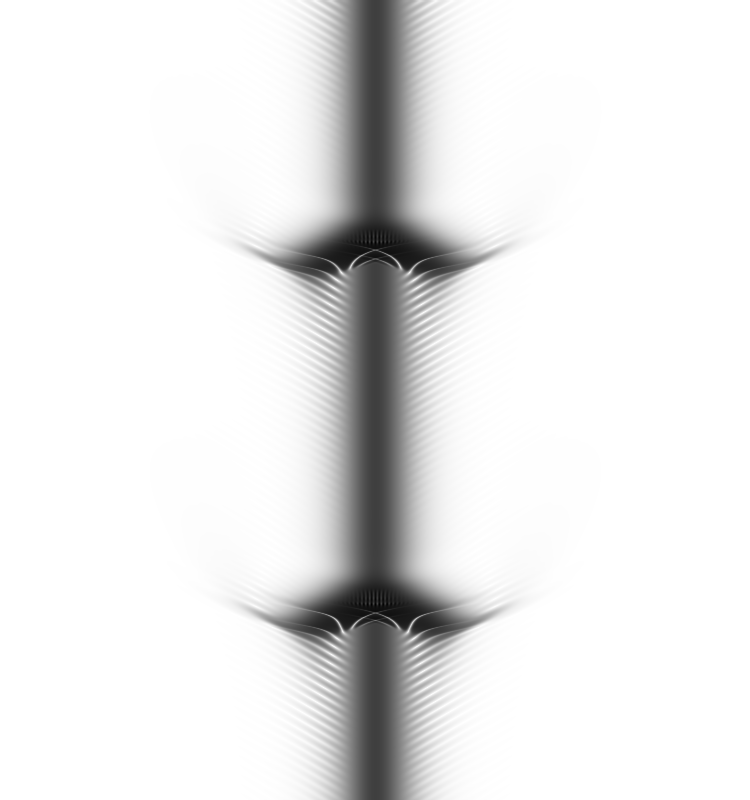
\includegraphics[width=2.6in]{expl}
\caption{The 2D intensity of an exploding soliton with parameters ..........}
\label{expl} 
\end{figure}
\begin{figure}[h]
\centering
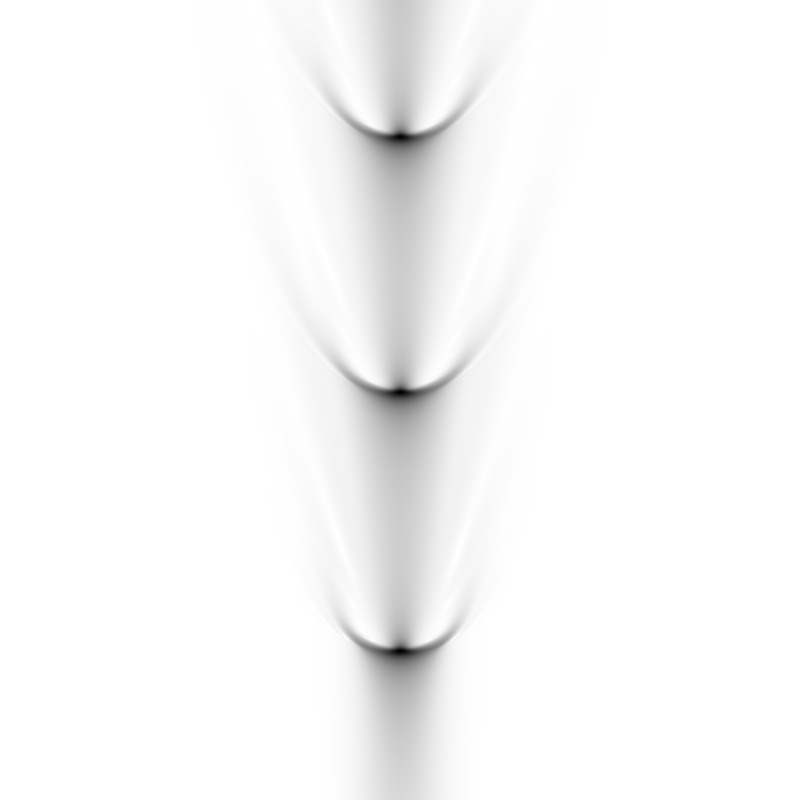
\includegraphics[width=2.6in]{highamp}
\caption{The 2D intensity of a high amplitude soliton with parameters ..........}
\label{highamp} 
\end{figure}
As parameters are varying, unusual behaviour can also be seen. 
For example, with the set of parameters (---------), when varying $\epsilon$, periodic doubling can be seen, as in figure \ref{periodic_doubling}. As the parameter c is increased, the the height of the solitons changes to a period 2 then a period 4 cycle. 
\begin{figure}[h]
\centering
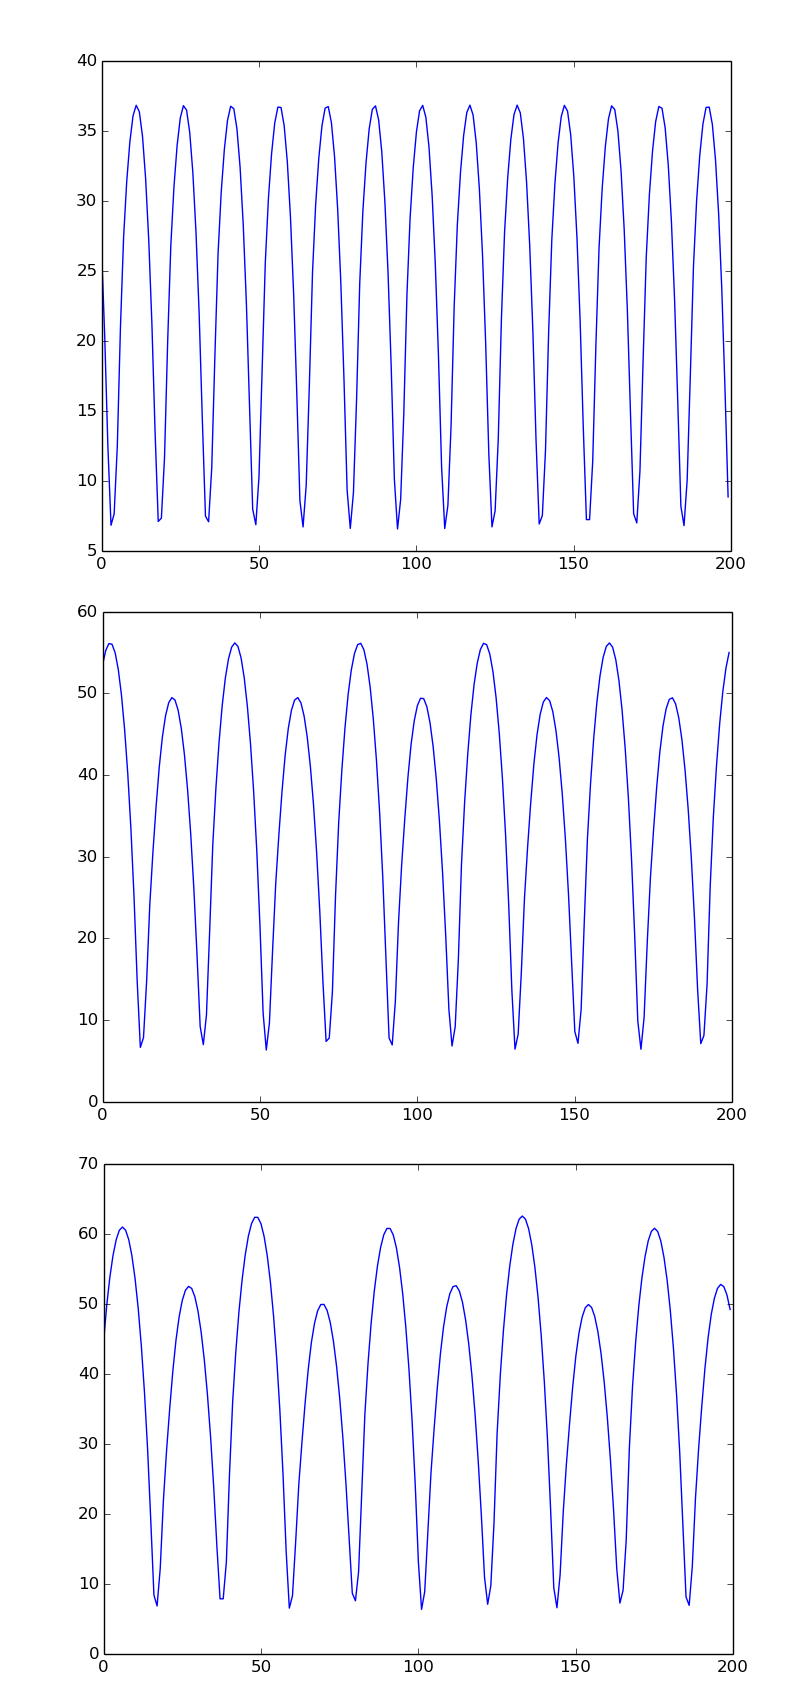
\includegraphics[width=2.6in]{periodic_doubling}
\caption{The energy profile of 3 solitons, with periodic doubling being seen. Parameters .........., for these images, the actual domain is from 0 to 100.}
\label{highamp} 
\end{figure}

We also get solitons that creep sideways as they oscillate.
An example is given in figure ------- of a soliton that creeps to the right forever. Another example is in figure \ref{periodpulse} 
\begin{figure}[h]
\centering
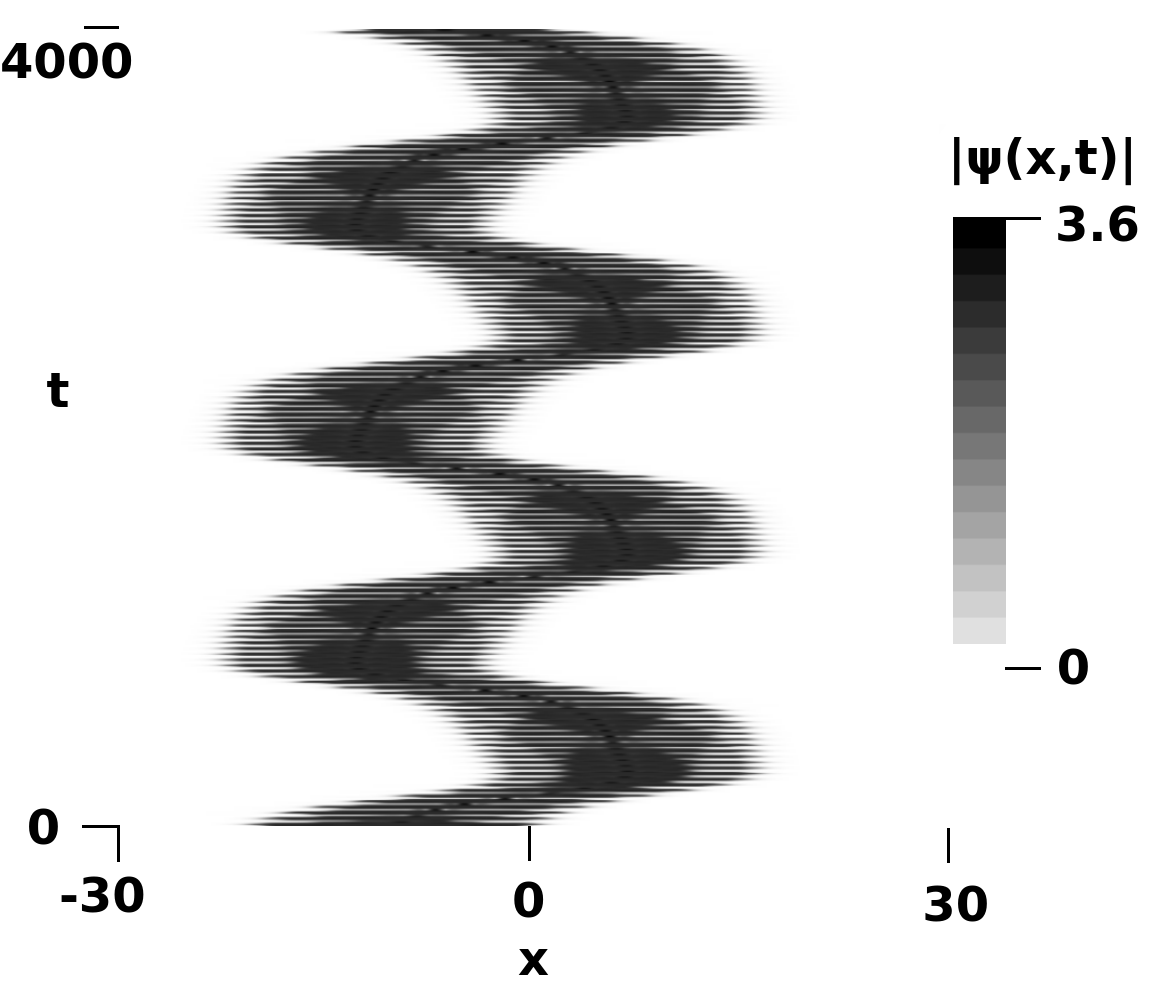
\includegraphics[width=2.6in]{periodpulse}
\caption{A creeping, pulseating soliton that is also periodic. Note that the weird patterning inside the image is from aliasing. params ---------}
\label{periodpulse} 
\end{figure}


\section{Previous things done to classify solitons in to regions}
The issue we have at the moment is that there are 6 parameters, and if we take 100 data points over a given range, we would need to calculate $10^12$ parameters. In addition, many parameters are given with high precision, and if we were to replicate this (high amplitude pulse), we would need many, many more points to plot. Given that each simulation takes a while with high precision, it is not an easy task to classify different regions, and typically has been done by hand and/or over a small region of space.
\\\\
Regions plotted are, for example, where exploding solitons occur, we get bifurcations in peak height. 









\chapter{Machine Learning Theory}
\section{Different Types of Machine Learning}
Very quickly summarise the MOOC.\\
I just need linear regression.

\section{Linear Regression}
Former Title: Different Options for the Machine Learning Algorithm\\
Another Title Removed: A detailed look at neural networks\\
\\
Step 1: Define a cost function:\\
Suppose we have input parameters $\vec x_i$ with the true value given by $y_i$. For linear regression, we choose $\vec\theta$ such that our prediction for the value of $y_i$ is $\vec\theta \cdot \vec x_i$. We want to vary the vector $\vec \theta$ such that the predictions match as best as possible. This is typically done by providing a cost function that is lowest when the predictions match the true value best. A typical cost function is (least squares):
$$J_\theta = \sum_i \left(\vec\theta\cdot \vec x_i -y_i\right)^2 $$
\\
Suppose we have two parameters, we might get an image as shown below. 
\begin{figure}[h]
\centering
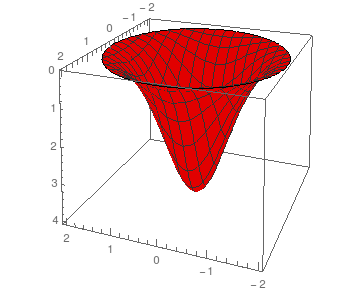
\includegraphics[width=3in]{GradDescent}
\caption{Gradient descent example}
\label{corr} 
\end{figure}
The minimum of this graph give $\theta$ which causes the best predictions. 
Typically the algorithm to find the minimum is done by continually taking the steepest path. However the algorithm may end up finding a local minima, as in the subsequent figure. 
\begin{figure}[h]
\centering
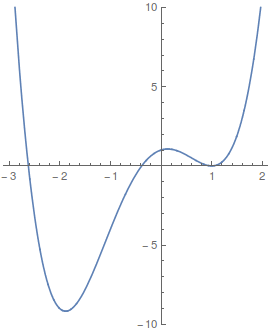
\includegraphics[width=2in]{localmin}
\caption{Gradient descent example}
\label{corr} 
\end{figure}
Octave has lots of fancy functions that can do this really efficiently, and can try to avoid local minima.
\\\\
We can increase the number of input features. One feature we want to add is an intercept term, which will equal $1$ for every training example. Other features we might want to add, for example, would be the polynomial features $\{x_1^2,x_1x_2,x_1x_3, ... \}$. However if we add in these extra features, we are faced with another issue, and that is overfitting. If we have a high degree polynomial, it becomes much easier to overfit the data. In order to prevent this, we can adjust the cost function to:
$$J_\theta = \frac{1}{2m}\sum_i \left(\vec\theta\cdot \vec x_i -y_i\right)^2 +\frac{\lambda}{2m} |\vec\theta|^2$$
By doing this, if several of the elements of $\vec \theta$ are large, then the cost will increase, and so only the important features will remain large. However for this to work we must normalise the data, and in my program this is done by transforming each feature $x_i^{(j)}$  in the following manner, where the $i$ indicates that it is the $i^{th}$ training example, and the $j$ index refers to the $j^{th}$ component of the vector. Below $\mu^{(j)}$ refers to the mean of the $j^{th}$ component of all the training examples, and $\sigma^{(j)}$ the standard deviation
$$x_i^{(j)}\rightarrow \frac{x_i^{(j)}-\mu^{(j)}}{\sigma^{(j)}}$$
This ensures that all of the features are on the same scale, and so the elements of $\theta$ are penalised equally by the cost function. 



\section{Training and Testing the Algorithm}

Tried initially with only linear terms, then expanded to polynomial terms with regularisation and it was able to fit data with polynomial features $(0.5x_1+x_2^3)$. This game me the confidence that the algorithm was working correctly, and so I could go ahead and train the algorithm on real data with confidence.\\\\
My algorithm went up to 4th order polynomial terms, and with 6 different parameters being varied, this results in a total of 210 features. 




\chapter{The result from much work}
\section{The sorts of things that I was looking for}
I now want to say something about what data I tested.\\
I took random parameters between (range) for all $\beta, \delta, D, \epsilon, \mu, \nu$\\
I ran the program for 350 time units with step size of 0.01. xrange = 40 with stepsize 0.01. Only the last 50 time units was kept so that it has time to stabilise into a stable soliton. 
\\\\
looking only at the last 50 time units to get this info.
Data recorded for each simulation: frequency of oscillation, max energy-min energy,  difference between max and min standard deviation, and height difference. Height difference is the maximum height minus the minimum height in that same column(i.e. if the maximum occurs in column 50, then we look for the minimum value in column 50)
\\\\
The freq is calculated by finding peaks in the energy profile, and taking the average distance between these peaks to be the period. Again, this is not neccessarily a constant, for example IMAGE.
\\\\
Once I have predicted things, plot the number within 5\% of the true value (and then 10\%, etc.). Keep in mind that I don't want all points matching well. For example, THIS IMAGE has multiple solitons being propagated forwards in time in parallel. This won't affect some things like period much, but it will effect the standard deviation. 
\\\\
\section{What was the accuracy?}
Plot the \% that was within $x$ from the true value (e.g. what percentage of the predicted frequency is within 5\%,10\%,15\% of the true value )

\section{Plots of regions}
Once this has been trained, plot the data for various regions, and compare with other other region plots that we have. (e.g. exploding vs normal solitons)





\unnum{chapter}{Conclusion}
\unnum{chapter}{Appendix A}
\unnum{chapter}{Appendix B}

\begin{thebibliography}{9}
%Introduction
\bibitem{RefExample}
    Name \emph{Title},
    Publishing info, etc
\bibitem{Ref2}
    Another Guy \emph{title2}
    pub,etc.
%Derivation of CGLE

%Types of Solitons

%Mathematical theory behind solving CGLE

%Machine Learning

%My solitons


\end{thebibliography}


\end{document}